\documentclass[border=2pt]{standalone}
\usepackage{circuitikz}
\begin{document}
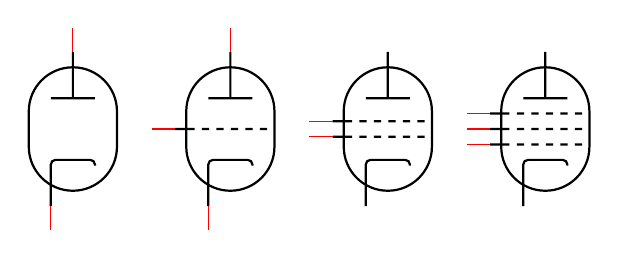
\begin{tikzpicture}
  \node[diodetube] (D) at (0,0) {};
  \node[triode] (T) at (2,0) {};
  \node[tetrode] (Q) at (4,0) {};
  \node[pentode] (P) at (6,0) {};
  \draw[red] (D.anode) -- ++(0,.3) (D.cathode) -- ++(0,-.3);
  \draw[red] (T.anode) -- ++(0,.3) (T.cathode) -- ++(0,-.3) (T.control) -- ++(-.3,0);
  \draw[red] (Q.control) -- ++(-.3,0) (Q.screen) -- ++(-.3,0);
  \draw[red] (P.control) -- ++(-.3,0) (P.screen) -- ++(-.3,0) (P.suppressor) -- ++(-.3,0);
\end{tikzpicture}
\end{document}
